\section{Exponentialfunktionen und Logarithmus}\label{sec:exponential}

\subsection{Exponentialfunktionen}
Exponentialfunktionen sind Funktionen der Form $f(x) = a^x$, wobei $a$ eine
konstante Zahl~$>0$ ist. Diese Funktionen haben einige gemeinsame
Eigenschaften:
\begin{itemize}
 \item $f(x) > 0$, d.~h. insbesondere die Funktion hat keine Nullstelle
 \item $f(0) = 1$, da $a^0 = 1$ für alle $a$
\end{itemize}

\begin{center}
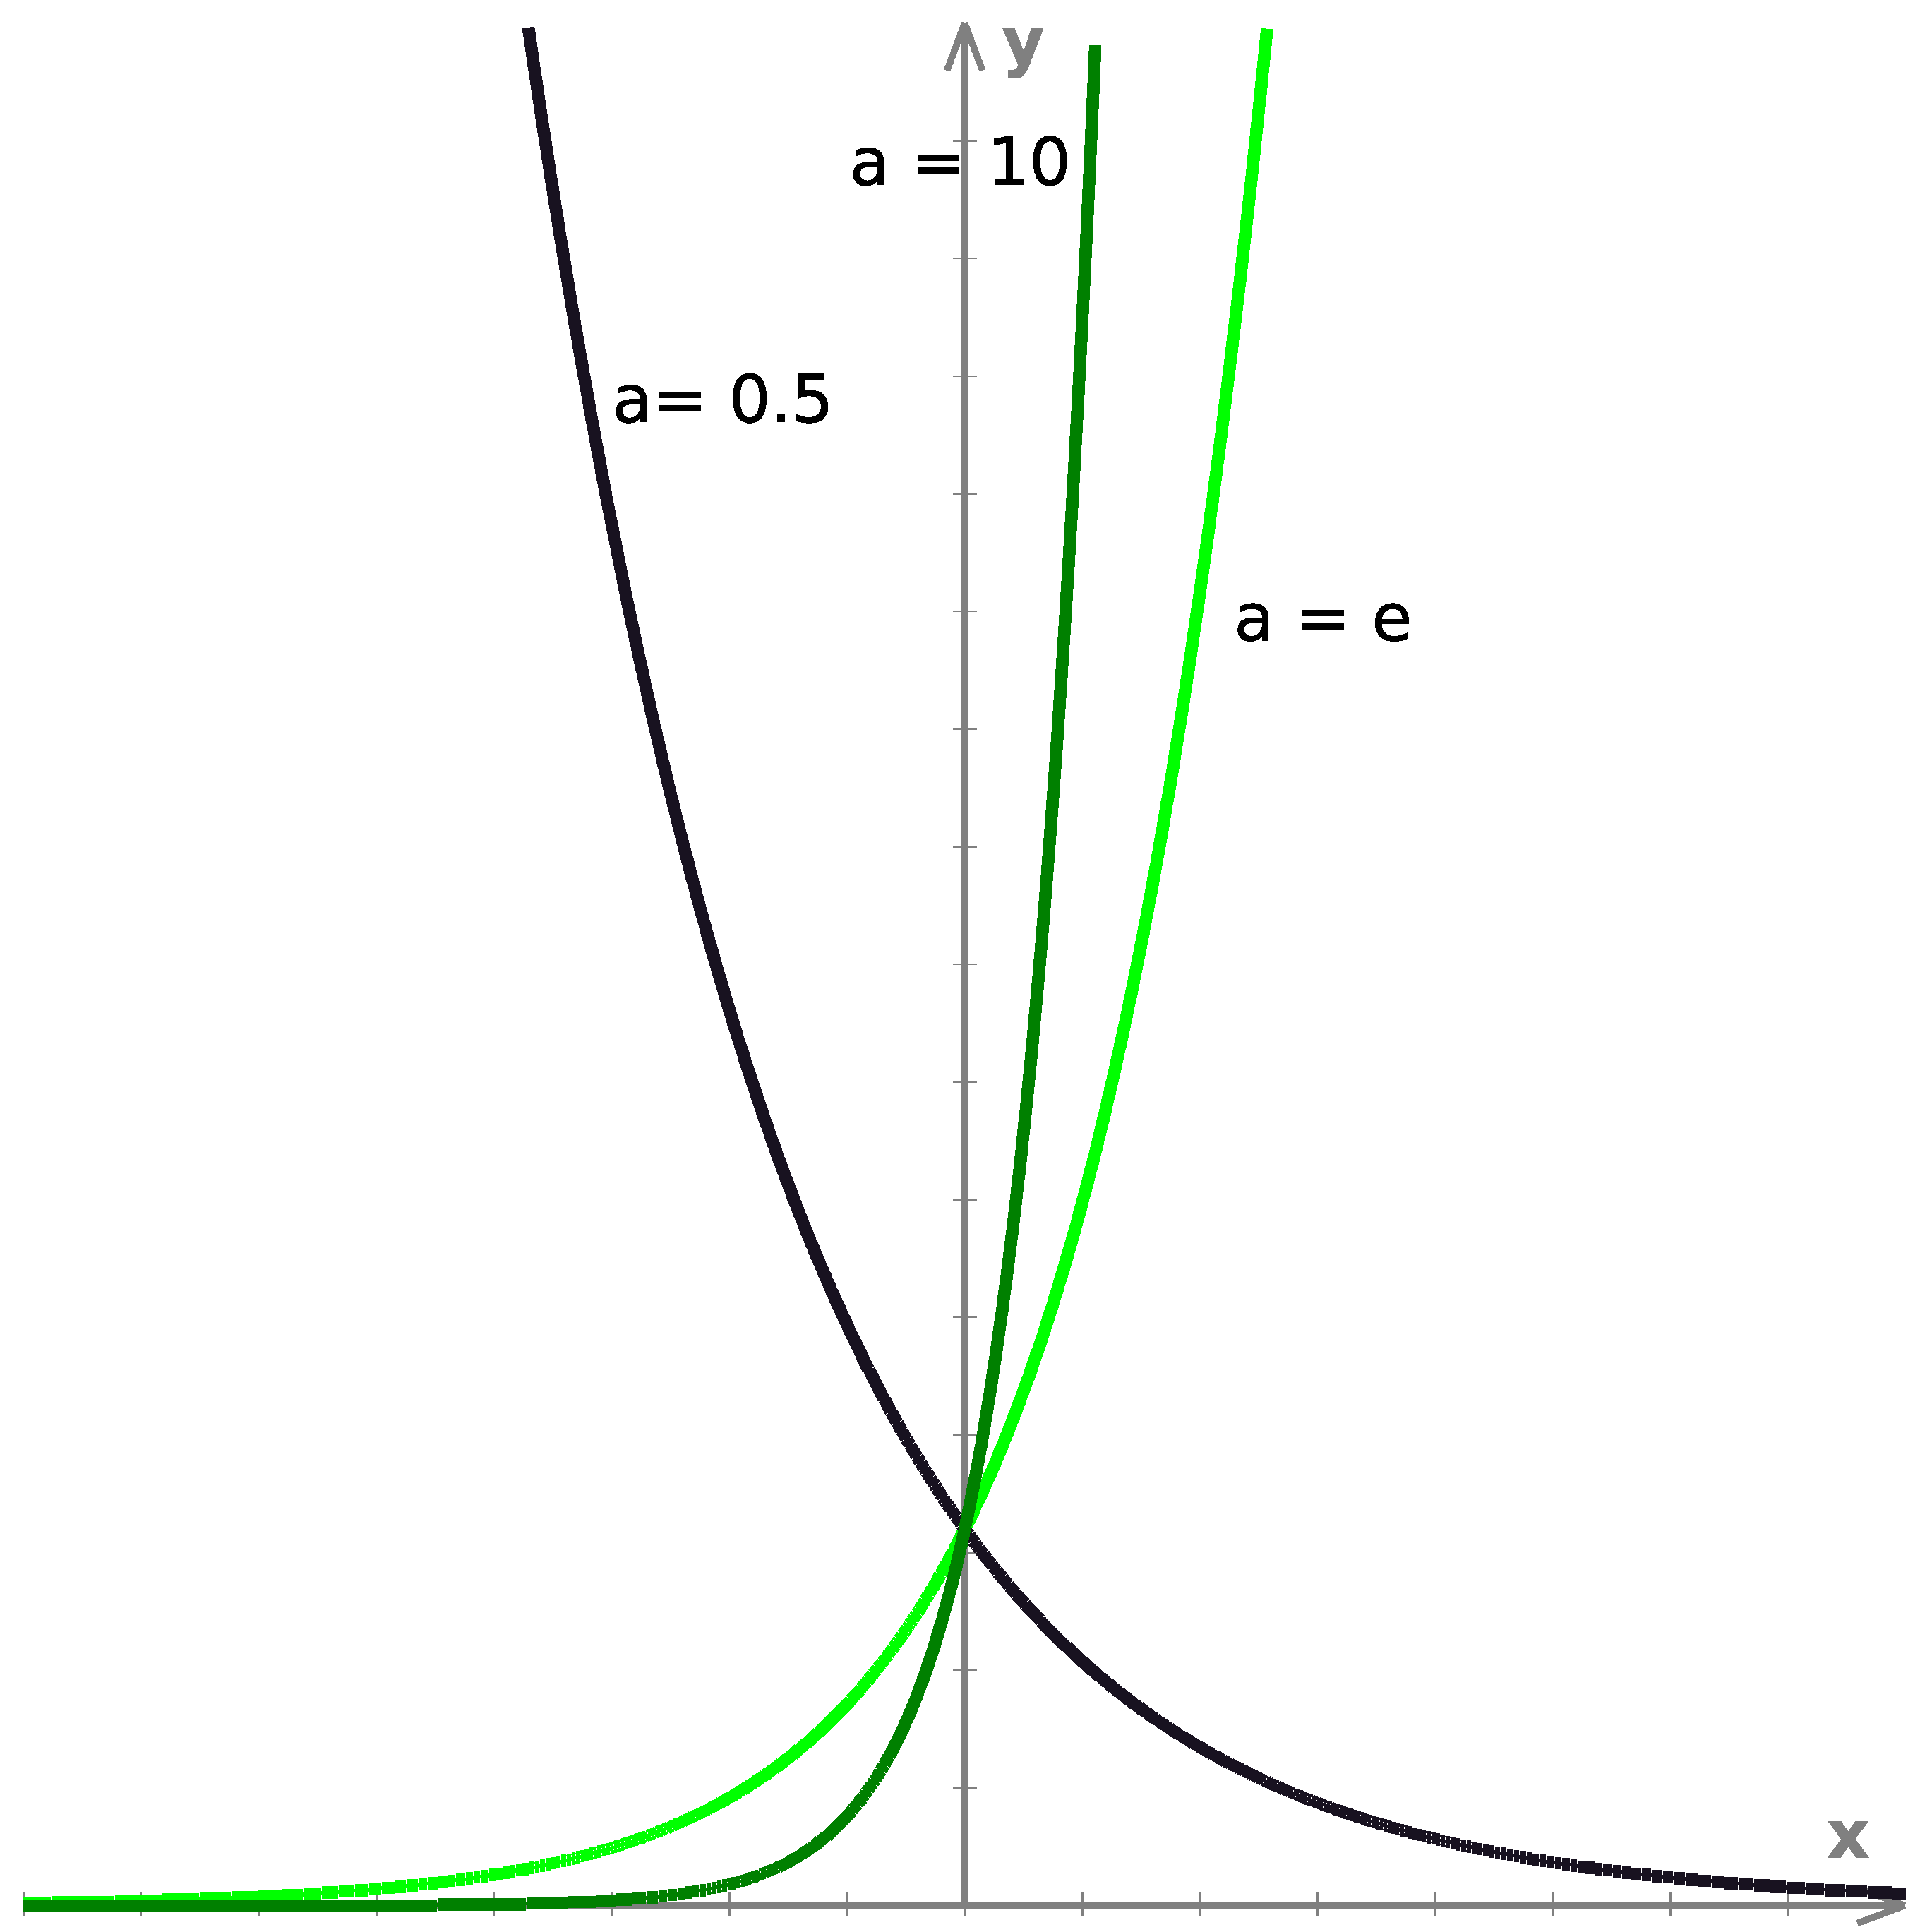
\includegraphics[width=.4\textwidth]{img/exp.pdf} 
\end{center}

\noindent Die Funktion hat abhängig von $a$ folgende Form:
\begin{description}
 \item[$\mathbf{a > 1}$] streng monoton wachsend, für $x \rightarrow -\infty$
geht $f(x)$ gegen $0$.
 \item[$\mathbf{0 < a < 1}$] streng monoton fallend, für $x \rightarrow
\infty$ geht $f(x)$ gegen $0$.
 \item[$\mathbf{a = 1}$] die Funktion ergibt konstant $1$ ($f(x) = 1^x$).
\end{description}

\noindent Eine spezielle Exponentialfunktion ist die $e$-Funktion $f(x) = e^x$, mit 
der sich viele natürliche Vorgänge beschreiben lassen. $e =
2,718281828459\dots$ ist die \emph{Eulersche Zahl}. Die $e$-Funktion hat die
Eigenschaft, dass $e^x = (e^x)' = (e^x)'' = (e^x)^{(n)}$, d.~h. alle Ableitungen der
Funktion sind gleich der Funktion.

\noindent Die Umkehrfunktion der Exponentialfunktionen ist der Logarithmus:
\[y = a^x \Longleftrightarrow x = \log_a y.\]


\subsection{Logarithmus}
Der Logarithmus $\log_a b$ (sprich: Logarithmus von $b$ zur Basis $a$) ist die
Zahl $c$, für die $a^c = b$ gilt. Der Logarithmus ist damit die
Umkehrfunktion der Exponentialfunktion.

\noindent Wichtige Logarithmen sind:

\begin{description}
 \item[Natürlicher Logarithmus] Logarithmus zur Basis $e$: $\log_e x = \ln x$
 \item[Dekadischer Logarithmus] Logarithmus zur Basis $10$: $\log_{10} x = \lg
x$ %(auf Taschenrechner: \emph{log})
 \item[Binärer Logarithmus] Logarithmus zur Basis $2$: $\log_2 x = \text{ld}\,
x$
\end{description}

\subsection{Logarithmusfunktion}
\begin{figure}
\begin{center}
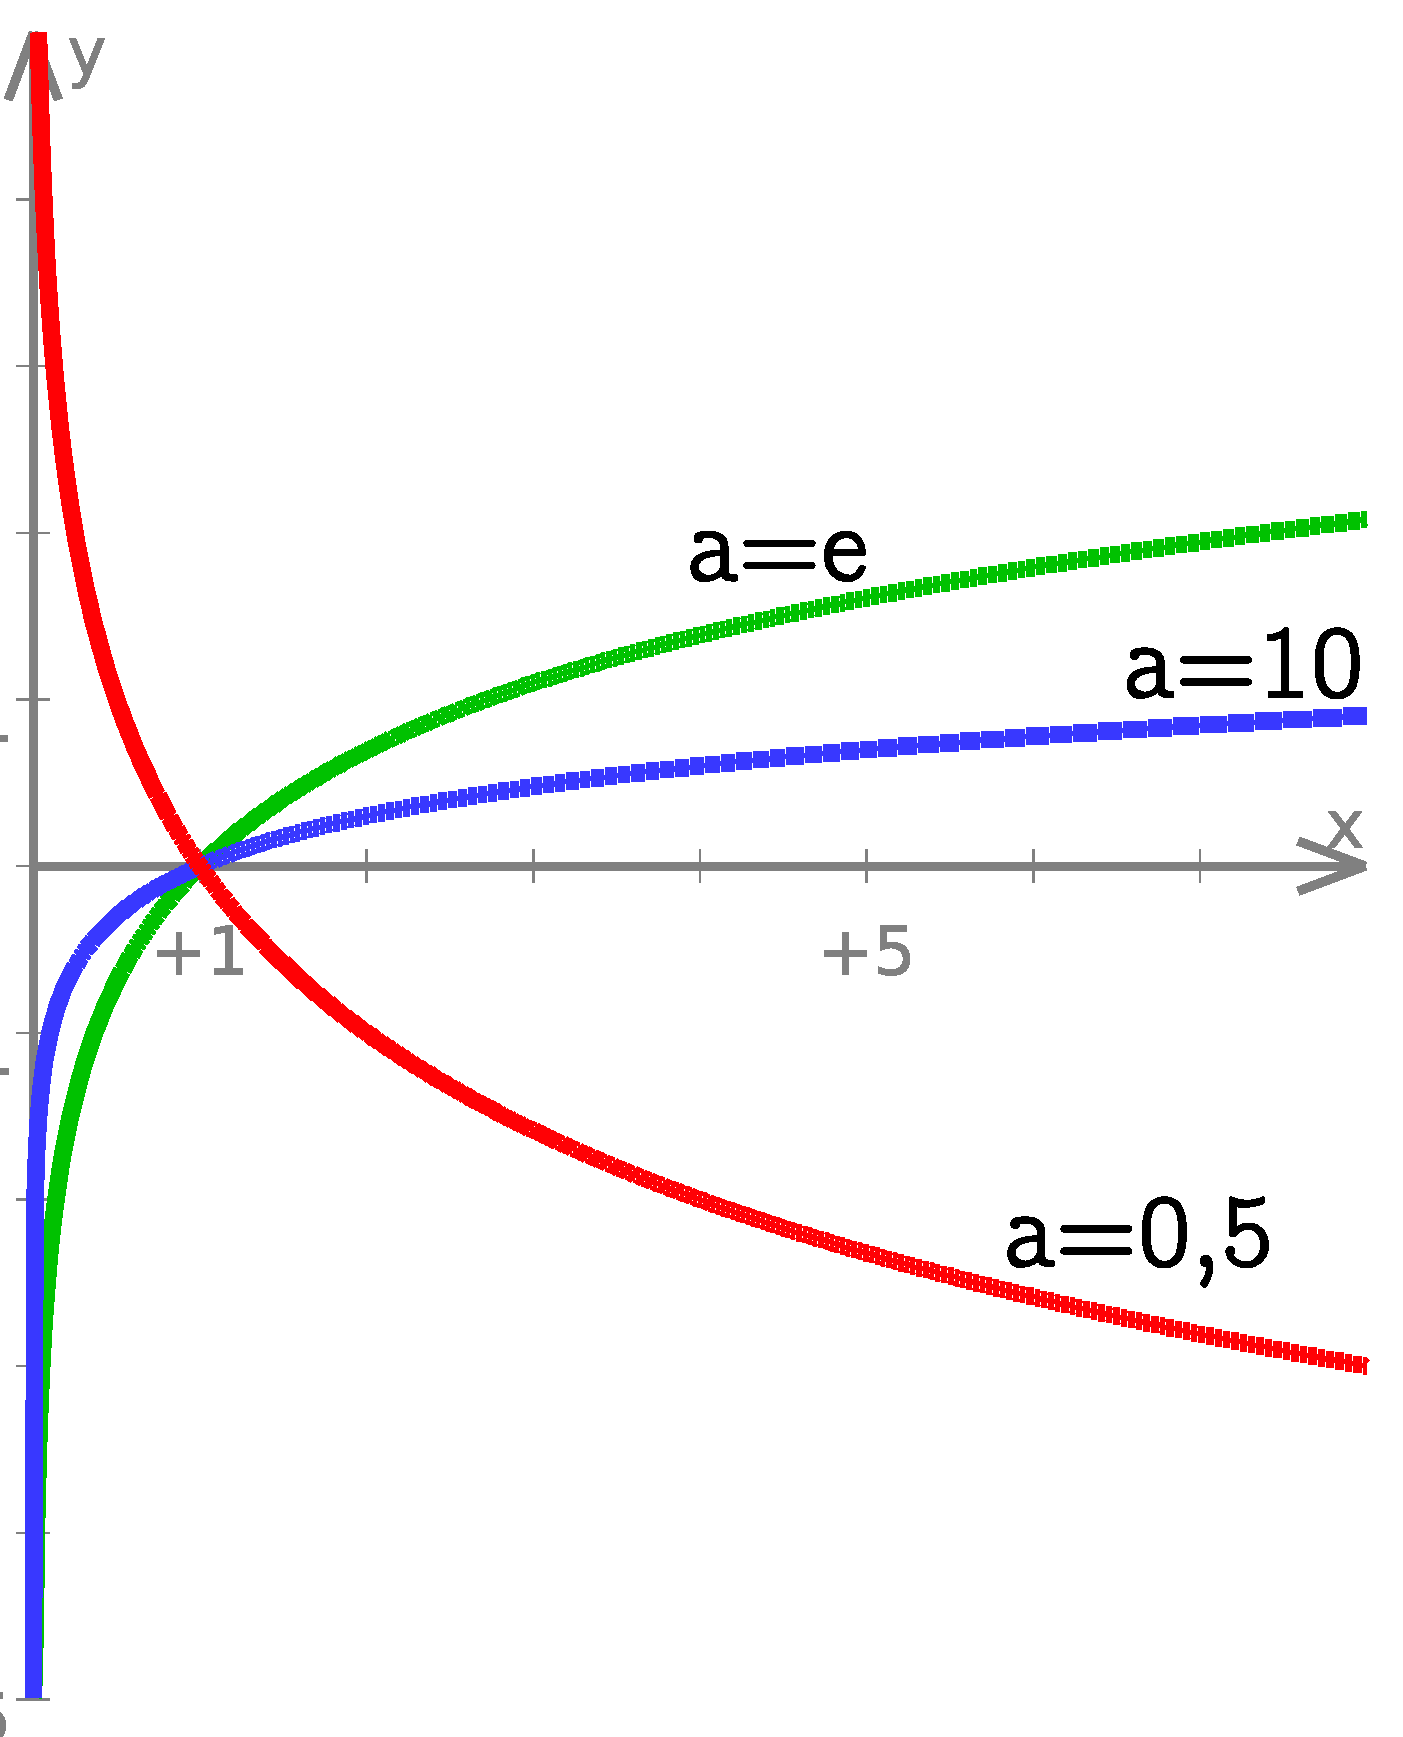
\includegraphics[height=4cm]{img/log.pdf}
\end{center}
\label{fig:logarithmus}
\caption{Graph der Funktion $\log_a x$, mit $a \in\{e, 10, \frac{1}{2}\}$.}
\end{figure}

Der Graph der Logarithmusfunktion (Abbildung 7.3) verhält sich ähnlich wie der Graph der
Exponentialfunktion: Abhängig von $a$ ist der Graph entweder monoton fallend
($0 < a < 1$) oder steigend ($a>1$). Die Funktion ist nur für positive Zahlen
definiert, der Grenzwert für $x \rightarrow 0$ ist $\pm\infty$. Der
Funktionswert $\log_a(1)$ ist $0$, unabhängig von $a$.
Für große Werte von $x$ (und $n > 0$) gilt: $log_a (x) < n\cdot x$, die Logarithmusfunktion wächst also langsamer als eine lineare Funktion.

\subsection{Logarithmengesetze}
\begin{eqnarray*}
\log_a(u\cdot v)  & = & \log_a u + \log_a v \\
\log_a\frac{u}{v} & = & \log_a u - \log_a v \\
\log_a u^r        & = & r\cdot \log_a u 
\end{eqnarray*}

\subsection{Basiswechsel}
Ein Logarithmus zu einer ungewöhnlichen Basis $a$ kann berechnen werden, indem
dieser auf eine andere Basis $b$ gebracht wird:
\[\log_a x = \frac{\log_b x}{\log_b a} \text{, z.~B. } \log_a x =
\frac{\ln x}{\ln a}\]

\noindent Dies ist nützlich, da die meisten Taschenrechner nur die Logarithmen
zur Basis $e$ (Taste \texttt{ln}) und $10$ (Taste \texttt{log}) berechnen
können. Alle anderen Logarithmen müssen auf diese Basen umgerechnet werden.


\subsection{Aufgaben}
\begin{enumerate}
 \item Löse nach $x$:
\begin{multicols}{3}
\begin{enumerate}
 \item $1 = e^x$
 \item $8 = 2^x$
 \item $3= 5e^x$
 \item $e = \frac{e^x}{e}$
 \item $9 = e^{cx}$
 \item $3 = \log_2 x$
 \item $0 = \log_{42} x$
 \item $0 = 5\log_5 x$
 \item $9 = 3\ln e^x$
\end{enumerate}
\end{multicols}

  \item Vereinfache:
  \begin{multicols}{2}
   \begin{enumerate}
    \item $\lg 2 +\lg 5$
    \item $\lg 5 +\lg 6 -\lg 3$
    \item $3\ln a +5\ln b -\ln c$
    \item $2\ln v - \ln v$
    \item $\frac{1}{2}\log_7 9 - \frac{1}{4}\log_7 81$
    \item $\log_3(x-4) + \log_3(x+4) = 3$
    \item $2 \log_2(4-x) + 4 = \log_2(x+5) - 1$ %32x^2 - 257x + 507 = 0
    \item $\log_5 x = \log_5 6 - 2  \log_5 3$ % x = 2/3
   \end{enumerate}
  \end{multicols}

  \item Das Wachstum von Bakterienkulturen lässt sich mit Hilfe der
$e$-Funktion beschreiben. Die Anzahl der Bakterien zum Zeitpunkt $t$ ist eine
Funktion $N(t)$, die abhängig ist von der anfänglichen Anzahl der Bakterien
(also der Wert $N_0 := N(0)$) und der Wachstumsrate $k$ des Bakteriums
(konstant). Es entsteht damit die Formel:
$N(t) = N_0e^{kt}$.

Für $N_0 = 100, k= 0,2$:
\begin{enumerate}
 \item Wieviele Bakterien gibt es zum Zeitpunkt 5 (10, 20, 50, 100)?
 \item Zu welchem Zeitpunkt gibt es 500 (1000, 5000, 10000) Bakterien?
\end{enumerate}

  \item Die Anzahl von Teilchen eines radioaktiven Materials ist ein
Exponentialfunktion der Zeit $N(t) = N_0e^{-\lambda t}$, wobei $N_0$ die
Anzahl der Teilchen zum Zeitpunkt 0 und $\lambda$ die Zerfallskonstante des
Materials ist. Gegen sind $N_0= 1000, \lambda = 2$.
\begin{enumerate}
  \item Wieviele Teilchen sind zum Zeitpunkt 1 (5, 10, 100) noch vorhanden?
  \item Wie lange dauert es, bis $\frac{1}{4}$ (die Hälfte (Halbwertszeit),
$\frac{3}{4}$, $\frac{7}{8}$) des Materials zerfallen ist?
\end{enumerate}

\end{enumerate}



\subsection{Literatur}
Frank, Schulz, Tietz, Warmuth: \textit{Wissenspeicher Mathematik}. 1. Auflg.
1998. Volk und Wissen Verlag Berlin. 
Weitere Formeln gibt es in der (umfangreichen) \emph{Formelsammlung
Trigonometrie} der Wikipedia\footnote{\url{http://de.wikipedia.org/wiki/Formelsammlung_Trigonometrie}}.

%%weiter siehe Kurvendiskussion